\chapter{Customization and Embedding}
\label{cha:opp-design}

\section{Architecture}

{\opp} has a modular architecture. The following diagram shows the
high-level architecture of {\opp} simulations:

\begin{figure}[htbp]
  \begin{center}
    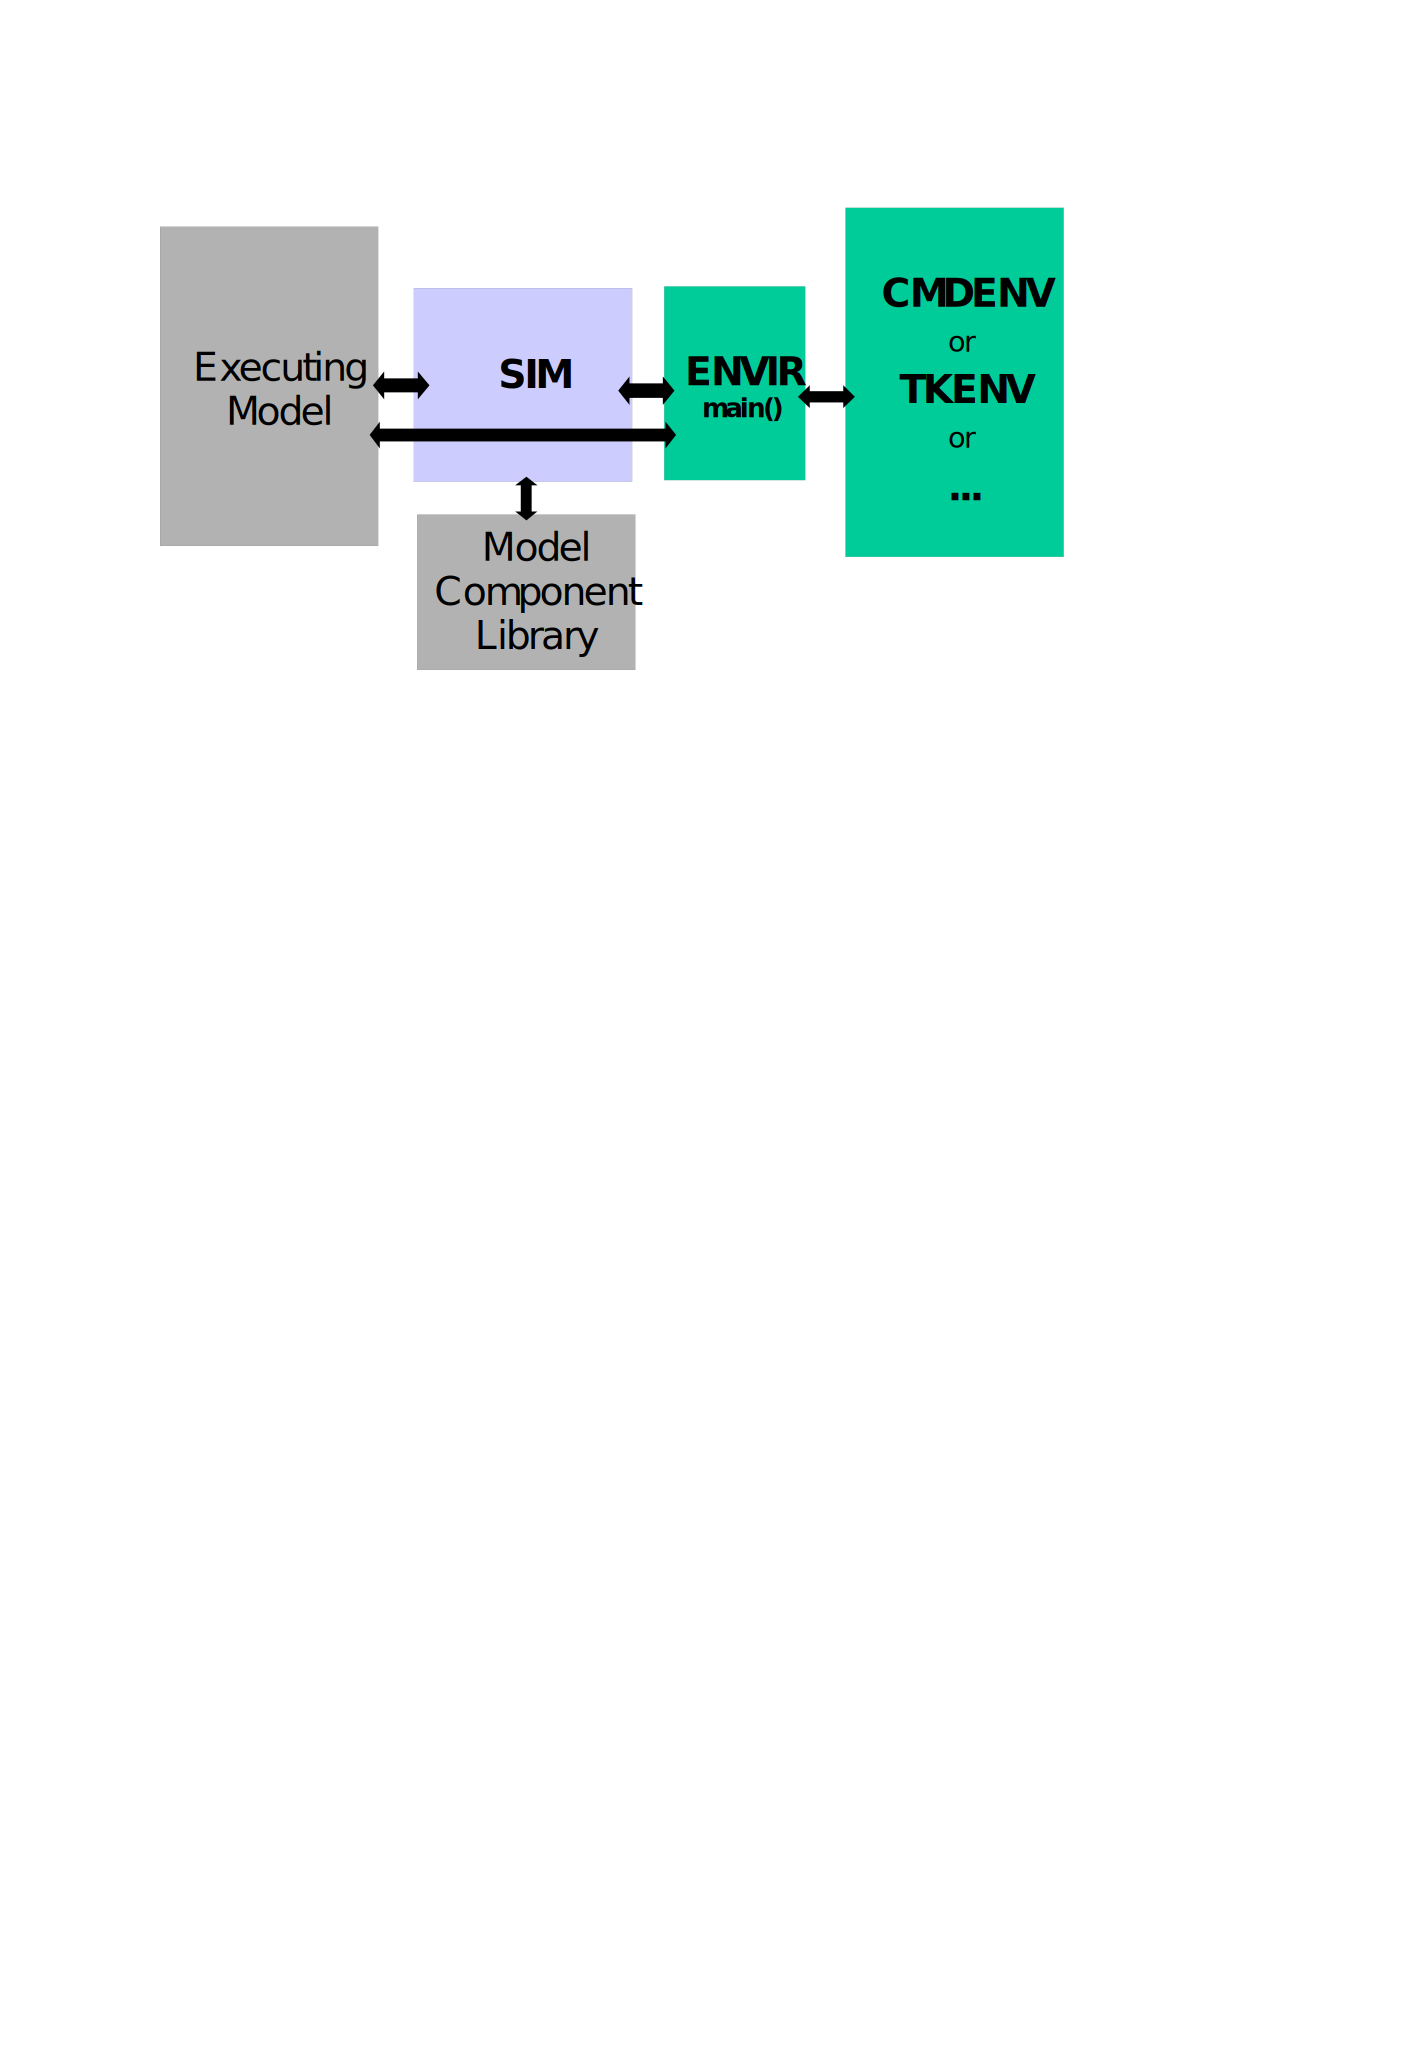
\includegraphics[width=4.757in, height=2.412in]{figures/usmanFig18}
    \caption{Architecture of {\opp} simulation programs}
  \end{center}
\end{figure}

The rectangles in the picture represent components:

\begin{itemize}
  \item{\textbf{Sim} is the simulation kernel and class
    library\index{simulation!kernel}. Sim exists as a library you link
    your simulation program with.
       \footnote{Use of dynamic (shared) libraries is also possible, but
       for simplicity we'll use the word \textit{linking} here.}
    }
  \item{\textbf{Envir} is another library which contains all code
    that is common to all user interfaces. \fname{main()} is also in Envir.
    Envir provides services like ini file handling for specific user interface
    implementations. Envir presents itself towards Sim and the executing model
    via the \ttt{ev} facade object, hiding all other user interface internals.
    Some aspects of Envir can be customized\index{customization} via plugin
    interfaces. Embedding {\opp} into applications\index{embedding} can
    be achieved implementing a new user interface in addition to Cmdenv and Tkev,
    or by replacing Envir with another implementation of \ttt{ev}
    (see sections \ref{sec:ch-opp-design:customization} and
    \ref{sec:ch-opp-design:embedding}.)}
  \item{\textbf{Cmdenv and Tkenv} are specific user interface
    implementations. A simulation is linked with
    either Cmdenv or Tkenv.}
  \item{The \textbf{Model Component Library} consists of simple module definitions and
    their C++ implementations, compound module types, channels, networks,
    message types and in general everything that belongs to models and
    has been linked into the simulation program. A simulation program is
    able to run any model that has all necessary components linked in.}
  \item{The \textbf{Executing Model} is the model that has been set up
    for simulation. It contains objects (modules, channels, etc.) that
    are all instances of components in the model component library.}
\end{itemize}

The arrows in the figure show how components interact with
each other:

\begin{itemize}
  \item{\textbf{Executing Model vs Sim}. The simulation kernel
    manages the future events and invokes modules in the executing model
    as events occur. The modules of the executing model are stored
    in the main object of Sim, \fvar{simulation} (of class \cclass{cSimulation}).
    In turn, the executing model calls functions in the
    simulation kernel and uses classes in the Sim library.}
  \item{\textbf{Sim vs Model Component Library}. The simulation kernel
    instantiates simple modules and other components when the simulation model
    is set up at the beginning of the simulation run. It also refers
    to the component library when dynamic module creation is used.
    The machinery for registering and looking up components in the model
    component library is implemented as part of Sim.}
  \item{\textbf{Executing Model vs Envir}. The \ttt{ev} object, logically
    part of Envir, is the facade of the user interface towards the executing model.
    The model uses \ttt{ev} to write debug logs (\ttt{ev<<}, \ttt{ev.printf()}).}
  \item{\textbf{Sim vs Envir}. Envir is in full command of what
    happens in the simulation program. Envir contains the \ttt{main()} function
    where execution begins. Envir determines which models should be set up
    for simulation, and instructs Sim to do so. Envir contains the main
    simulation loop (\textit{determine-next-event}, \textit{execute-event}
    sequence) and invokes the simulation kernel for the necessary
    functionality (event scheduling and event execution are implemented in Sim).
    Envir catches and handles errors and exceptions that occur
    in the simulation kernel or in the library
    classes during execution. Envir presents a single facade object (\ttt{ev})
    that represents the environment (user interface) toward Sim -- no Envir
    internals are visible to Sim or the executing model.
    During simulation model setup, Envir supplies parameter values for
    Sim when Sim asks for them. Sim writes output vectors via Envir,
    so one can redefine the output vector storing mechanism by changing Envir.
    Sim and its classes use Envir to print debug information.}
  \item{\textbf{Envir vs Tkenv and Cmdenv}. Envir defines \cclass{TOmnetApp}
    as a base class for user interfaces, and Tkenv and Cmdenv both subclass
    from \cclass{TOmnetApp}. The \ttt{main()} function provided as part of Envir
    determines the appropriate user interface class (subclassed from
    \cclass{TOmnetApp}), creates an instance and runs it -- whatever
    happens next (opening a GUI window or running as a command-line program)
    is decided in the \ttt{run()} method of the appropriate \cclass{TOmnetApp}
    subclass. Sim's or the model's calls on the \ttt{ev} object are
    simply forwarded to the \cclass{TOmnetApp} instance. Envir presents
    a framework and base functionality to Tkenv and Cmdenv via the methods of
     \cclass{TOmnetApp} and some other classes.)}
\end{itemize}


\section{Embedding {\opp}}
\label{sec:ch-opp-design:embedding}

This section discusses the issues of embedding the simulation kernel
or a simulation model into a larger application.

What you'll absolutely need for a simulation to run is the Sim library. You
probably do not want to keep the appearance of the simulation program, so
you do not want Cmdenv and Tkenv. You may or may not want to keep Envir.
You can keep Envir if its philosophy and the infrastructure it provides
(\ttt{omnetpp.ini}, certain command-line options etc.) fit into your
design. Then your application, the embedding program will take the place of
Cmdenv and Tkenv.

If Envir does not fit your needs (for example, you want the model
parameters to come from a database not from \ttt{omnetpp.ini}), then you
have to replace it. Your Envir replacement (the embedding application,
practically) must implement the \cclass{cEnvir} member functions from
\ttt{envir/cenvir.h}, but you have full control over the simulation.

Normally, code that sets up a network or builds the internals of a
compound module comes from compiled NED source.  You may not like the
restriction that your simulation program can only simulate networks
whose setup code is linked in. No problem; your program can contain
pieces of code similar to what is currently generated by nedc and then it can build
any network whose components (primarily the simple modules) are linked
in. Moreover, it is possible to write an integrated environment where
you can put together a network using a graphical editor and right
after that you can run it, without intervening NED compilation and
linkage.





\section{Sim: the simulation kernel and class library}

There is little to say about Sim here, since chapters
\ref{cha:simple-modules} and \ref{cha:the-simulation-library},
and part of chapter \ref{cha:messages} are all about
this topic. Classes covered in those chapters are documented
in more detail in the API Reference generated by Doxygen.
What we can do here is elaborating on some internals
that have not been covered in the general chapters.

The source code for the simulation kernel\index{simulation!kernel}
and class library reside in the \ttt{src/sim/} subdirectory.


\subsection{The global simulation object}

The global \ttt{simulation} object is an instance of \cclass{cSimulation}.
It stores the model, and encapsulates much of the functionality
of setting up and running a simulation model.

\ttt{simulation} has two basic roles:

\begin{itemize}
  \item{it stores modules of the executing model}
  \item{it holds the future event set (FES) object}
\end{itemize}



\subsection{The coroutine package}

The coroutine package is in fact made up of two coroutine
packages\index{coroutine}:

\begin{itemize}
  \item A portable coroutine package creates all coroutine stacks
     inside the main stack. It is based on Kofoed's solution\cite{Kofoed95}.
     It allocates stack by deep-deep recursions and then plays with
     \fname{setjmp()} and \fname{longjmp()} to switch from one to another.

  \item On Windows, the Fiber functions (\fname{CreateFiber()},
     \fname{SwitchToFiber()}, etc) are used, which are part of
     the standard Win32 API.
\end{itemize}

The coroutines are represented by the \cclass{cCoroutine}
class. \cclass{cSimpleModule} has \cclass{cCoroutine} as one a
base class.



\section{The Model Component Library}

All model components (simple module definitions and their C++
implementations, compound module types, channels, networks,
message types, etc.) that you compile and link into a simulation
program are registered in the Model Component Library.
Any model that has all its necessary components in the
component library of the simulation program can be run by that
simulation program.

If your simulation program is linked with Cmdenv or Tkenv,
you can have the contents of its component library printed,
using the -h switch.

\begin{verbatim}
% ./fddi -h

OMNeT++ Discrete Event Simulation  (C) 1992-2004 Andras Varga
...
Available networks:
  FDDI1
  NRing
  TUBw
  TUBs

Available modules:
  FDDI_MAC
  FDDI_MAC4Ring
  ...

Available channels:
  ...
End run of OMNeT++
\end{verbatim}

Information on components are kept on registration lists.
There are macros for registering components (that is, for adding
them to the registeration lists):
\ttt{\fmac{Define\_Module()}}, \ttt{\fmac{Define\_Module\_Like()}},
\ttt{\fmac{Define\_Network()}}, \ttt{\fmac{Define\_Function()}},
\fmac{Register\_Class()}, and a few others. For components defined
in NED files, the macro calls are generated by the NED compiler;
in other cases you have to write them in your C++ source.

Let us see the module registrations as an example. The

\begin{verbatim}
Define_Module(FIFO);
\end{verbatim}

macro expands to the following code:

\begin{verbatim}
static cModule *FIFO__create(const char *name, cModule *parentmod)
{
    return new FIFO(name, parentmod);
}

EXECUTE_ON_STARTUP( FIFO__mod,
    modtypes.instance()->add(
       new cModuleType("FIFO","FIFO",(ModuleCreateFunc)FIFO__create)
    );
)
\end{verbatim}

When the simulation program starts up, a new \cclass{cModuleType}
object will be added to the \ttt{modtypes} object, which holds the list
of available module types. The \cclass{cModuleType} object will act as a factory:
when its create() method is called it will produce a new module object
of class \ttt{FIFO} via the above static function \ttt{FIFO\_\_create}.

The \ttt{cModuleType} object also stores the name of the corresponding
NED module declaration. This makes it possible to add the gates and parameters
declared in NED to the module when it is created.

The machinery for managing the registration lists are part
of the Sim library. Registration lists are implemented
as global objects.

The registration lists are:

\begin{longtable}{|p{2cm}|p{4,3cm}|p{7.3cm}|}
\hline
%% ROW 1
\tabheadcol
\textbf{List variable}
&
\textbf{Macro/}\linebreak
\textbf{Objects on list}
&
\textbf{Function} \\\hline
%% ROW 2
\ttt{networks}
&
\ttt{\fmac{Define\_Network()}} \linebreak
\linebreak
\ttt{\cclass{cNetworkType}}
&
{\raggedright List of available networks\index{network!list of}.
A \cclass{cNetworkType} object holds a pointer to a function that can
build up the network.
\fmac{Define\_Network()} macros occur in the code generated by the NED
compiler.}\\\hline
% ROW 3
\ttt{modtypes}
&
\ttt{\fmac{Define\_Module()},} \linebreak
\ttt{\fmac{Define\_Module\_Like()},}  \linebreak
\linebreak
\ttt{\cclass{cModuleType}}
&
{\raggedright List of available module types.
A \cclass{cModuleType} object knows how to create a module of a specific
type. If it is compound, it holds a pointer to a function that can
build up the inside.
Usually, \fmac{Define\_Module()} macros for compound modules occur in
the code generated by the NED compiler; for simple modules,
the \fmac{Define\_Module()} lines are added by the user.}\\\hline
%% ROW 4
\ttt{classes}
&
\fmac{Register\_Class()} \linebreak
\linebreak
\ttt{cClassRegister}
&
{\raggedright List of available classes of which one can create
an instance.
A \cclass{cClassRegister} object has a ``factory method'' for creating an object
of a specific class. The list is used by the \fname{createOne()} function:
it can create an object of any class, given the class name as a string.
(E.g. the statement \ttt{ptr = createOne("cArray")} creates a \ttt{cArray} object.)
To enable a class to work with \ttt{createOne()}, one has to register it using the
\ttt{Register\_Class(classname)} macro}\\\hline
%% ROW 5
\ttt{functions}
&
\ttt{\fmac{Define\_Function()}} \linebreak
\linebreak
\ttt{\cclass{cFunctionType}}
&
{\raggedright List of functions taking \ttt{double}s and returning a \ttt{double}
(see type \ttt{MathFuncNoArg}...\ttt{MathFunc3Args}).
A \cclass{cFunctionType} object holds a pointer to the function and knows
how many arguments it takes.}\\\hline
%% ROW 6
\ttt{linktypes}
&
\fmac{Define\_Link()} \linebreak
\linebreak
%FIXME this is obsolete!!!!!!!!
\cclass{cLinkType}
&
{\raggedright List of link types.
A \cclass{cLinkType} object knows how to create \cclass{cPar} objects representing
the delay\index{channel!delay}, error\index{channel!error} and datarate\index{channel!datarate} attributes for a channel.
\fmac{Define\_Link()} macros occur in the code generated by the NED
compiler, one for each channel definition.} \\\hline
\end{longtable}





\section{Envir, Tkenv and Cmdenv}

The source code for the user interface of {\opp} resides in the
\texttt{src/envir/} directory (common part) and in the \texttt{src/cmdenv/},
\texttt{src/tkenv/} directories.

The classes in the user interface are \textit{not} derived from \cclass{cObject},
they are completely separated from the simulation kernel.



\subsection{The main() function}

The \fname{main()} function of {\opp} simply sets up the user
interface and runs it. Actual simulation is done in
\fname{cEnvir::run()} (see later).



\subsection{The cEnvir interface}

The \cclass{cEnvir} class has only one instance, a global object
called \fvar{ev}:

\begin{verbatim}
cEnvir ev;
\end{verbatim}

\cclass{cEnvir} basically a facade, its member functions
contain little code. \cclass{cEnvir} maintains a pointer to a
dynamically allocated simulation application object (derived from
\cclass{TOmnetApp}, see later) which does all actual work.


\cclass{cEnvir} member functions perform the following groups of tasks:
\begin{itemize}
  \item I/O for module activities; the actual implementation is different
    for each user interface (e.g. stdin/stdout for Cmdenv, windowing
    in Tkenv)
  \item cEnvir provides methods for the simulation kernel to
    access configuration information (for example, module parameter settings)
  \item cEnvir also provides methods that are called by simulation kernel to
    notify the user interface of certain events (an object was deleted;
    a module was created or deleted; a message was sent or delivered, etc.)
\end{itemize}


\subsection{Customizing Envir}
\label{sec:ch-opp-design:customization}

Certain aspects of Envir can be customized via plugin interfaces.
Plugin interfaces are presented in the form of C++ abstract classes
that you have to implement, register via the \fmac{Register\_Class()}
macro, and finally tell Envir to use them via \ttt{omnetpp.ini} entries.

The following plugin interfaces are supported:

\begin{itemize}
   \item{\cclass{cRNG}. Interface for the random number generator.}
   \item{\cclass{cScheduler}. The scheduler class. This plugin interface
     allows for implementing real-time, hardware-in-the-loop, distributed
     and distributed parallel simulation.}
   \item{\cclass{cConfiguration}. It defines a class
     from which all configuration will be obtained. In other words, it
     option lets you replace \ttt{omnetpp.ini} with some other implementation,
     e.g. database input.}
   \item{\cclass{cOutputScalarManager}. It handles recording the scalar output data,
     output via the cModule::recordScalar() family of functions.
     The default output scalar manager is \cclass{cFileOutputScalarManager},
     defined in the Envir library.}
   \item{\cclass{cOutputVectorManager}. It handles recording the output
     for \cclass{cOutVector} objects.
     The default output vector manager is \cclass{cFileOutputVectorManager},
     defined in the Envir library.}
   \item{\cclass{cSnapshotManager}. It provides an output stream to which
     snapshots are written (see section \ref{sec:ch-sim-lib:snapshots}).
     The default snapshot manager is \cclass{cFileSnapshotManager},
     defined in the Envir library.}
\end{itemize}

The above interfaces are documented in the API Reference.

The corresponding ini file entries that allow you to select your
plugin classes are \fpar{configuration-class}, \fpar{scheduler-class},
\fpar{rng-class}, \fpar{outputvectormanager-class},
\fpar{outputscalarmanager-class} and \fpar{snapshotmanager-class},
documented in section \ref{sec:ch-run-sim:general-section}.

\subsubsection{How plugin classes can access the configuration}

The configuration is available to plugin classes via the \fname{config()}
method of \cclass{cEnvir}, which returns a pointer to the configuration
object (\cclass{cConfiguration}). This enables plugin classes to have
their own config entries.

An example which reads the \ttt{parsim-debug} boolean entry from the
\ttt{[General]} section, with \ttt{true} as default:

\begin{verbatim}
bool debug = ev.config()->getAsBool("General", "parsim-debug", true);
\end{verbatim}


\subsubsection{Startup sequence for the configuration plugin}

For the configuration plugin, the startup sequence is the following
(see \ttt{cEnvir::setup()} in the source code):

\begin{enumerate}
  \item First, \ttt{omnetpp.ini} (or the ini file(s) specified via the "-f"
     command-line option) are read.
  \item Shared libraries in \ttt{[General]/load-libs} are loaded.
     (Also the ones specified with the "-l" command-line option.)
  \item \ttt{[General]/configuration-class} is examined, and if it is present,
     a configuration object of the given class is instantiated.
     The configuration object may read further entries from the
     ini file (e.g. database connect parameters, or XML file name).
  \item The original \ttt{omnetpp.ini} \cclass{cInifile} configuration
     object is deleted. No other settings are taken from it.
  \item \ttt{[General]/load-libs} from the new configuration object is
     processed.
  \item Then everything goes on as normally, using the new configuration
     object.
\end{enumerate}

%FIXME cScheduler usage


\subsection{Implementation of the user interface: simulation applications}

The base class for simulation application is \cclass{TOmnetApp}.
Specific user interfaces such as \cclass{TCmdenv},
\cclass{TOmnetTkApp} are derived from \cclass{TOmnetApp}.

\cclass{TOmnetApp}'s member functions are almost all virtual.
\begin{itemize}
  \item{Some of them implement the \cclass{cEnvir} functions
    (described in the previous section)}
  \item{Others implement the common part of all user interfaces (for
    example: reading options from the configuration files; making the
    options effective within the simulation kernel)}
  \item{The \fname{run()} function is pure virtual (it is different
    for each user interface).}
\end{itemize}

\cclass{TOmnetApp}'s data members:
\begin{itemize}
  \item{a pointer to the object holding configuration file contents
    (type \cclass{cInifile});}
  \item{the options and switches that can be set from the
    configuration file (these members begin with \ttt{opt\_})}
\end{itemize}

Simulation applications:
\begin{itemize}
  \item{add new configuration options}
  \item{provide a \fname{run()} function}
  \sloppy
  \item{implement functions left empty in \cclass{TOmnetApp} (like
    \fname{breakpointHit()}, \fname{objectDeleted()}).}
\end{itemize}


%
% section{Writing inspectors for TkEnv}
%
% TBD
%

%%% Local Variables:
%%% mode: latex
%%% TeX-master: "usman"
%%% End:
